\documentclass{scrartcl}

\usepackage[utf8]{inputenc}
\usepackage[T1]{fontenc}
\usepackage{lmodern}
\usepackage[english]{babel}
\usepackage{amsmath}
\usepackage{graphicx}
\usepackage{caption}	
\usepackage{subcaption}	 
\usepackage{hyperref}
\usepackage[parfill]{parskip}
\usepackage{hhline}
\usepackage{subcaption}

\title{Neuroprosthetics - Exercise 7}
\author{Alexander Koenig}
\date{26. January 2019}

\begin{document}
\maketitle

\section{Border Frequencies of a Filter}

The simplified Cochlear Implant (CI) consists of $n \in \{3, 6, 12, 22\}$ electrodes and uses a bandpass filter for each electrode on the array. The border frequencies of each electrode are logarithmically distributed between an overall range of 100Hz for the most apical electrode to 8 kHz for the most basal electrode. Below is a list of the border frequencies (in Hz) for each electrode array. Figure \ref{fig:borderf_22} shows a logarithmic plot of the border frequencies of a cochlear implant with 22 electrodes. 
\begin{itemize}
	\item $n=3$:	 [ 100.  431. 1857. 8000.]
	\item $n=6$: 	 [ 100.  208.  431.  894. 1857. 3854. 8000.]
	\item $n=12$: 	 [ 100.  144.  208.  299.  431.  621.  894. 1289. 1857. 2675. 3854. 5553.
 8000.]
 	\item $n=22$: 	 [ 100.  122.  149.  182.  222.  271.  330.  403.  492.  601.  733.  894.
 1092. 1332. 1626. 1984. 2421. 2955. 3606. 4401. 5371. 6555. 8000.]
\end{itemize}


\begin{figure}[h]
	\centering
	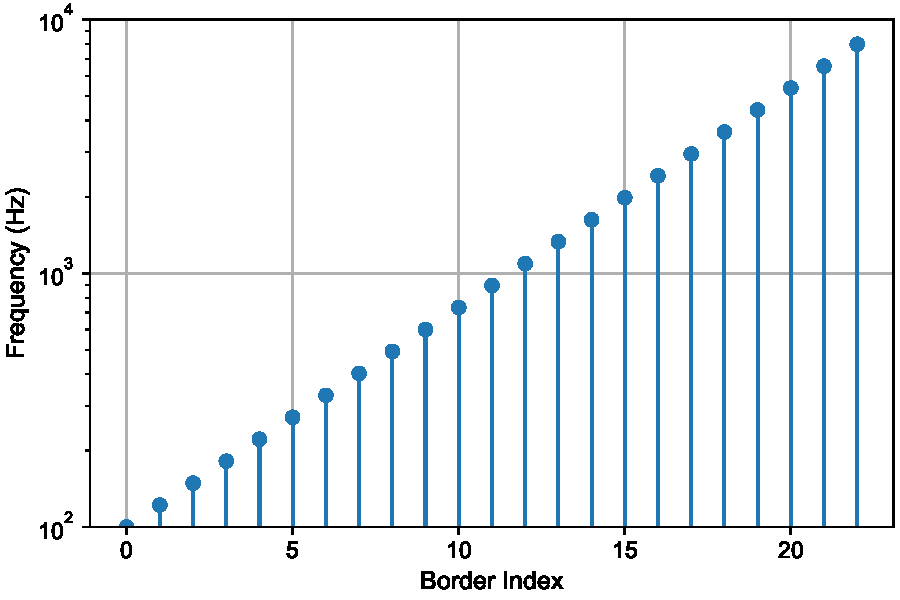
\includegraphics[width=0.65\textwidth]{figures/borders_CI_22}
	\caption{Border frequencies of CI with 22 electrodes}
	\label{fig:borderf_22}
\end{figure}

\newpage
\section{Implement a Filter Bank}
A second-order bandpass filter bank was implemented for the cochlear implants with the above border frequencies using the Butterworth bandpass filter. Butterworth filters feature a cutoff frequency of $-3.01$dB at the border frequencies and a maximally flat filter response in the passband. When viewed on a logarithmic plot the response rolls off linearly towards negative infinity at a rate of $-12$dB per octave for second-order filters. Figure \ref{fig:f_3} and \ref{fig:f_22} show the frequency response of the filter bank for 3 and 22 electrodes respectively. 

The phrase "Koenig's Test Word" was recorded with a microphone and filtered with the filter banks. The time signal of each filter channel of a 12-electrode CI is plotted in figure \ref{fig:filtered_all}. The blue lines represent the original sample, whereas the orange plot represents the sound at the electrode. By investigating the plotted results and by listening to each filter channel it becomes evident that some electrodes can represent specific spoken letters. For example, electrodes 1 to 4 mainly catch the lower sound of the "oe" in "Koenig's Test Word". The highly pitched "s" sounds in the words are captured by electrode 12. Here three distinct peaks in the signal at both "s" sounds and at the "t" can be identified. 

\newpage

\begin{figure}[h]
	\centering
	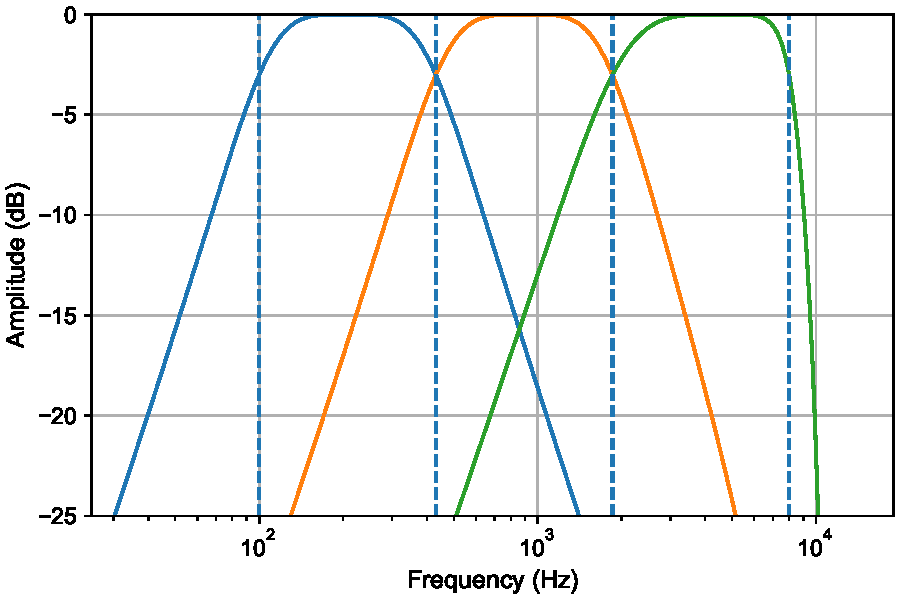
\includegraphics[width=0.8\textwidth]{figures/freq_response_CI_3}
	\caption{Frequency response for 3-electrode filter bank}
	\label{fig:f_3}
\end{figure}
\begin{figure}[h!]
	\centering
	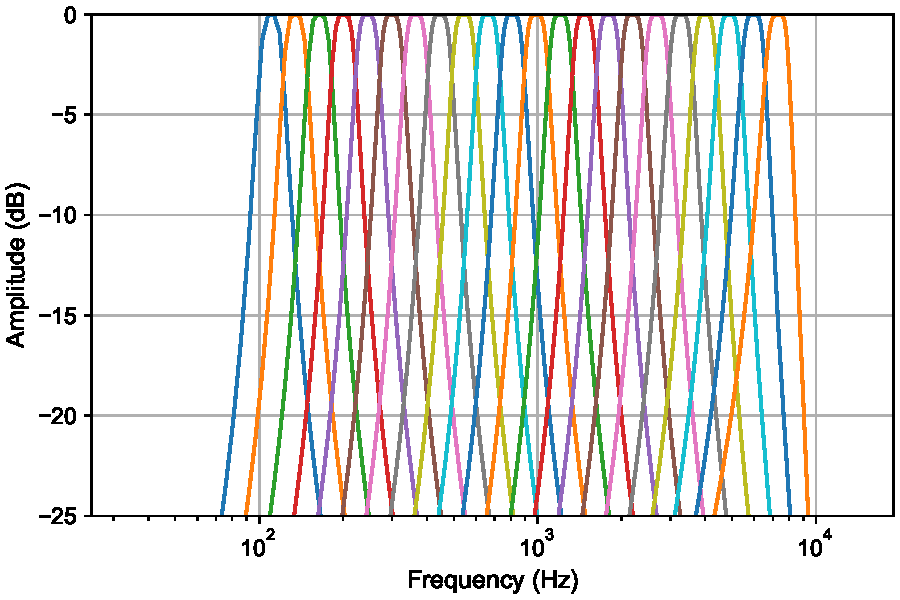
\includegraphics[width=0.8\textwidth]{figures/freq_response_CI_22}
	\caption{Frequency response for 22-electrode filter bank}
	\label{fig:f_22}
\end{figure}

\begin{figure}[p]
	\centering
	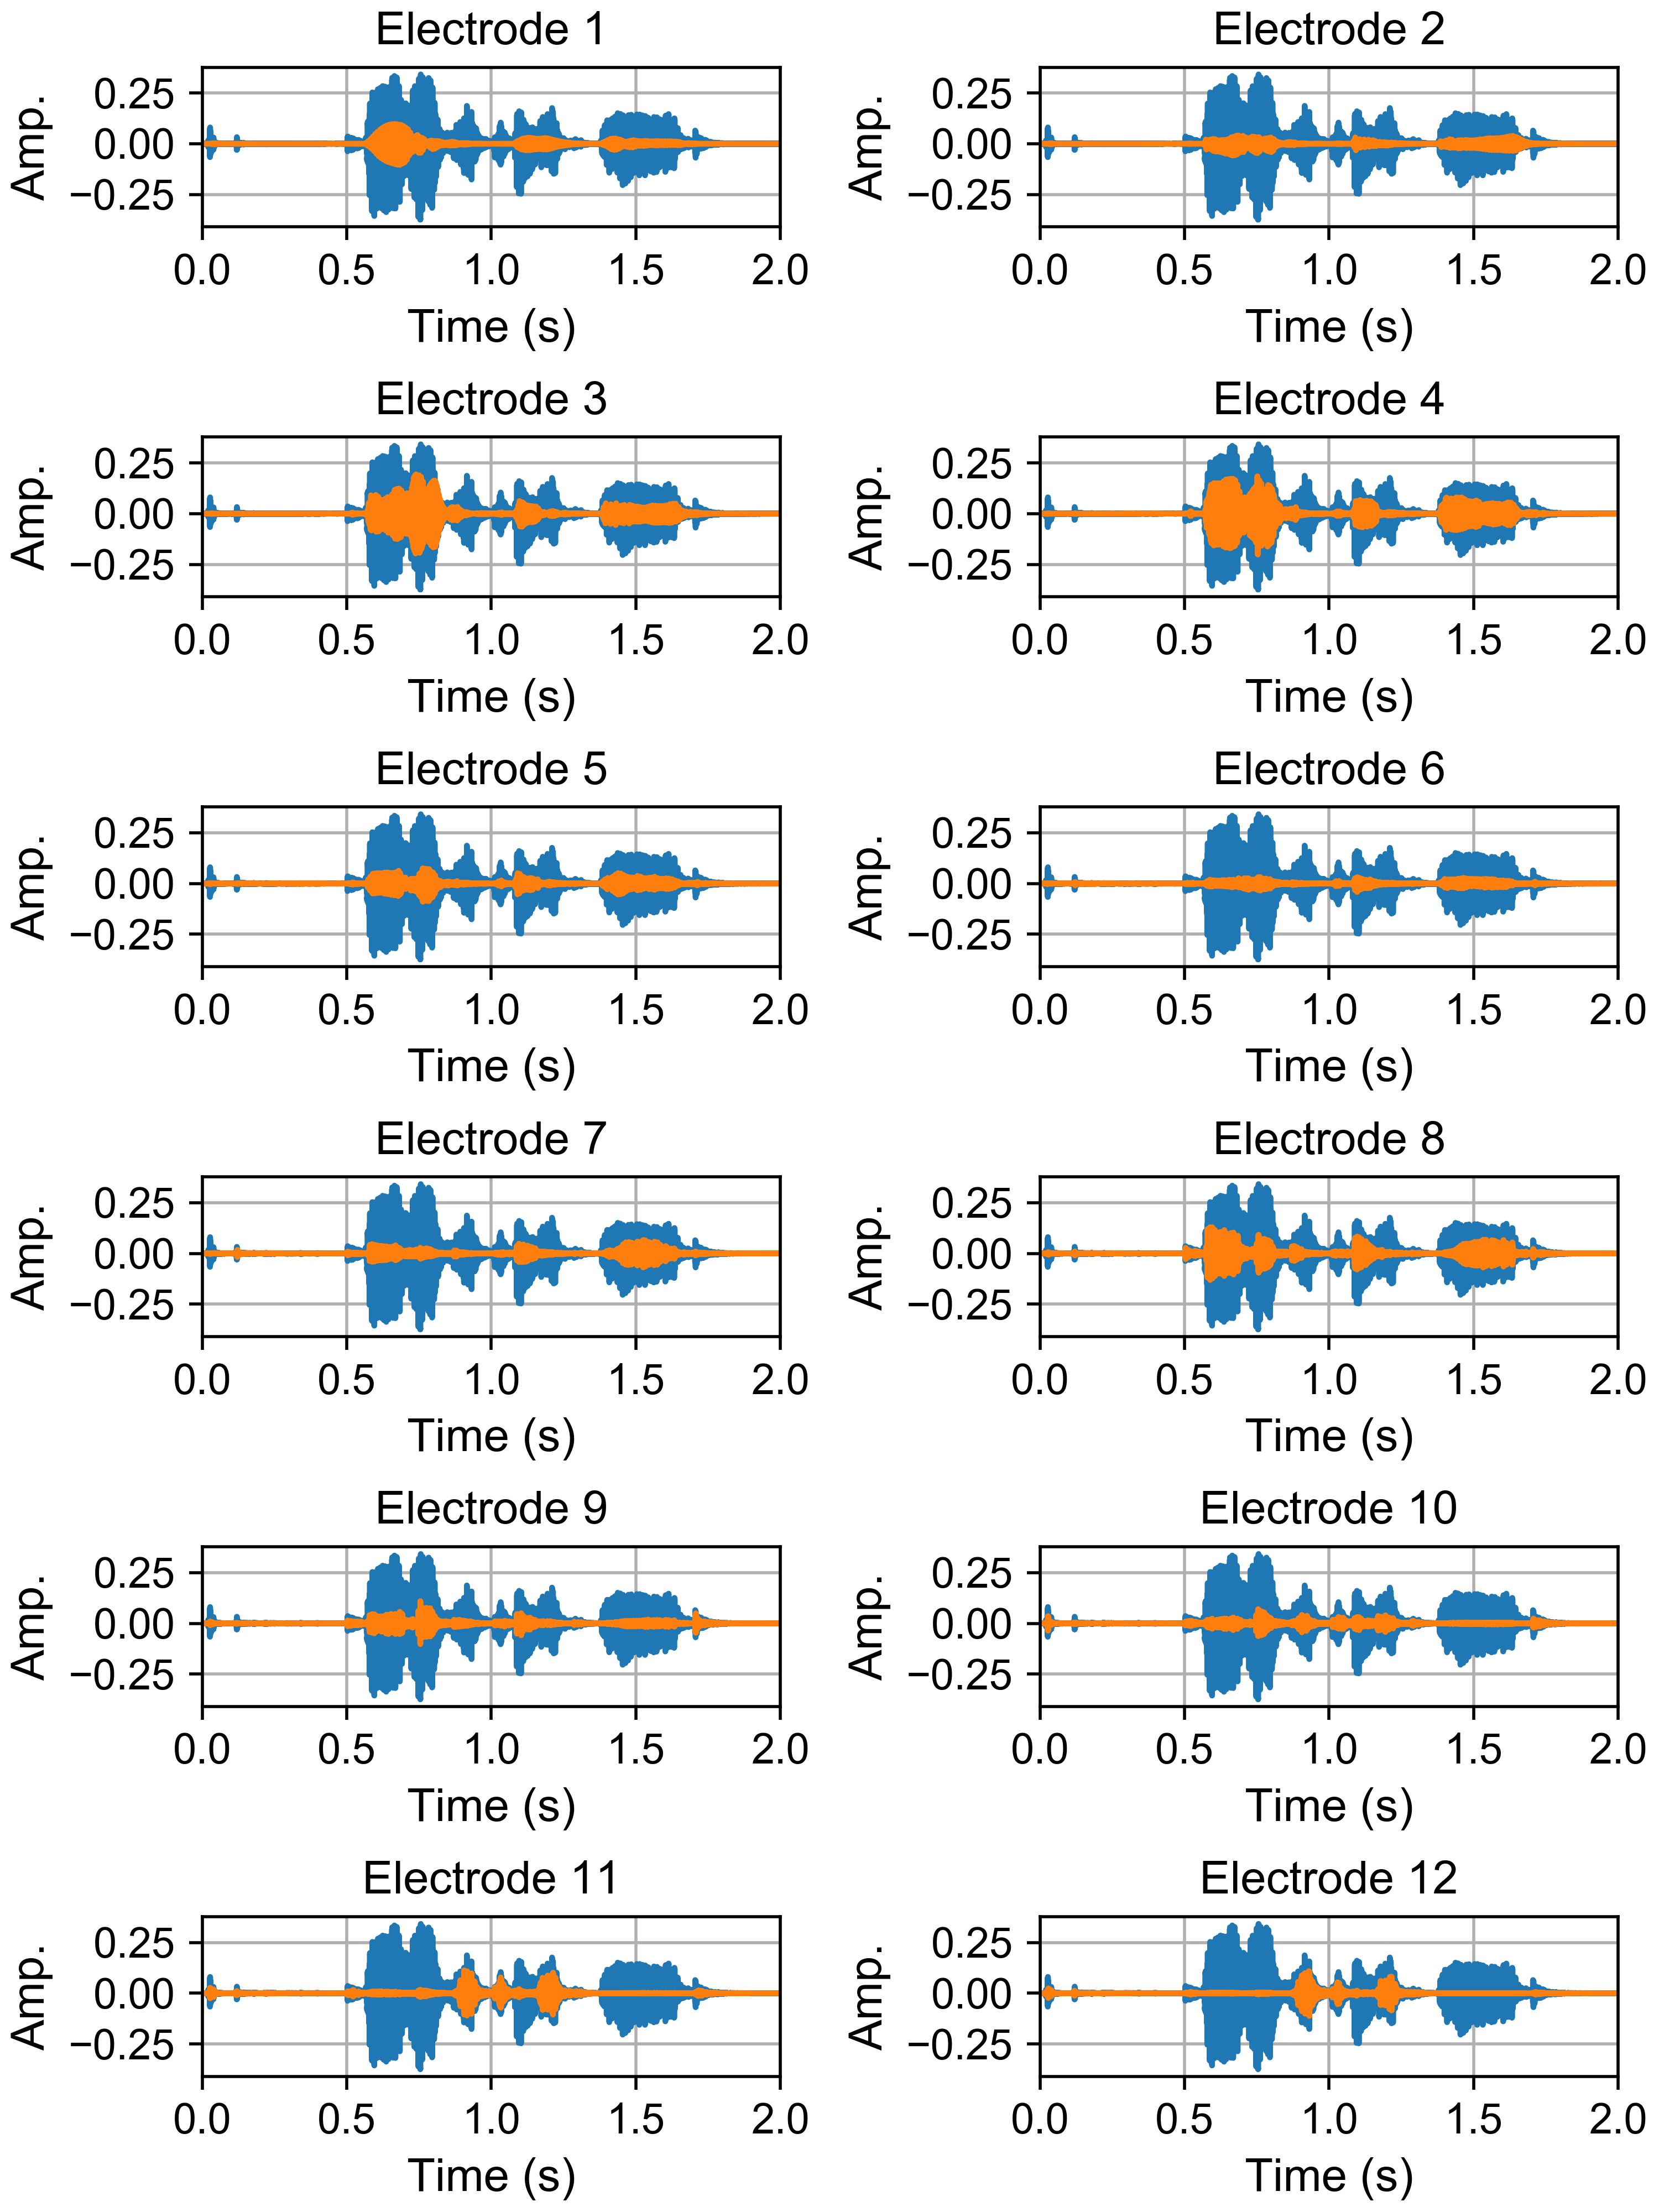
\includegraphics[width=0.95\textwidth]{figures/filtered_all}
	\caption{Amplitude at each electrode}
	\label{fig:filtered_all}
\end{figure}

\newpage
\section{Join the Channels}

In this section, the individual signals at each electrode are summed back together in order to compare them to the original signal. For reference figures \ref{fig:amplitude_koenigstestword}, \ref{fig:spectrum_koenigstestword} and \ref{fig:spectrogram_koenigstestword} show the amplitude, spectrum and spectrogram of the original signal, respectively. Figures \ref{fig:amplitude_sum}, \ref{fig:spectra} and \ref{fig:spectrograms} display the same data for each CI, but this time reconstructed from the electrode array of the cochlear implant. When one listens to the summed output of the electrode array the signal can almost not be distinguished from the original sound, even for the CI with 3 electrodes. 

The similarity of the signals can also be seen from the spectrograms - they are almost identical for each CI. The reason for this is that the whole audible spectrum is covered by the filters. In the spectrogram, one can observe each of the three words ("Koenig's", "Test", "Word") as a distinct area. 

From figure \ref{fig:spectra} it becomes clear that the higher the number of electrodes, the more power is lost. This may be due to the fact that there are more border areas which are attenuated by -3dB. This effect can also be observed in the amplitude plots in figure \ref{fig:amplitude_sum} where the amplitude of the signals decreases the more electrodes there are.

\begin{figure}[h]
	\centering
	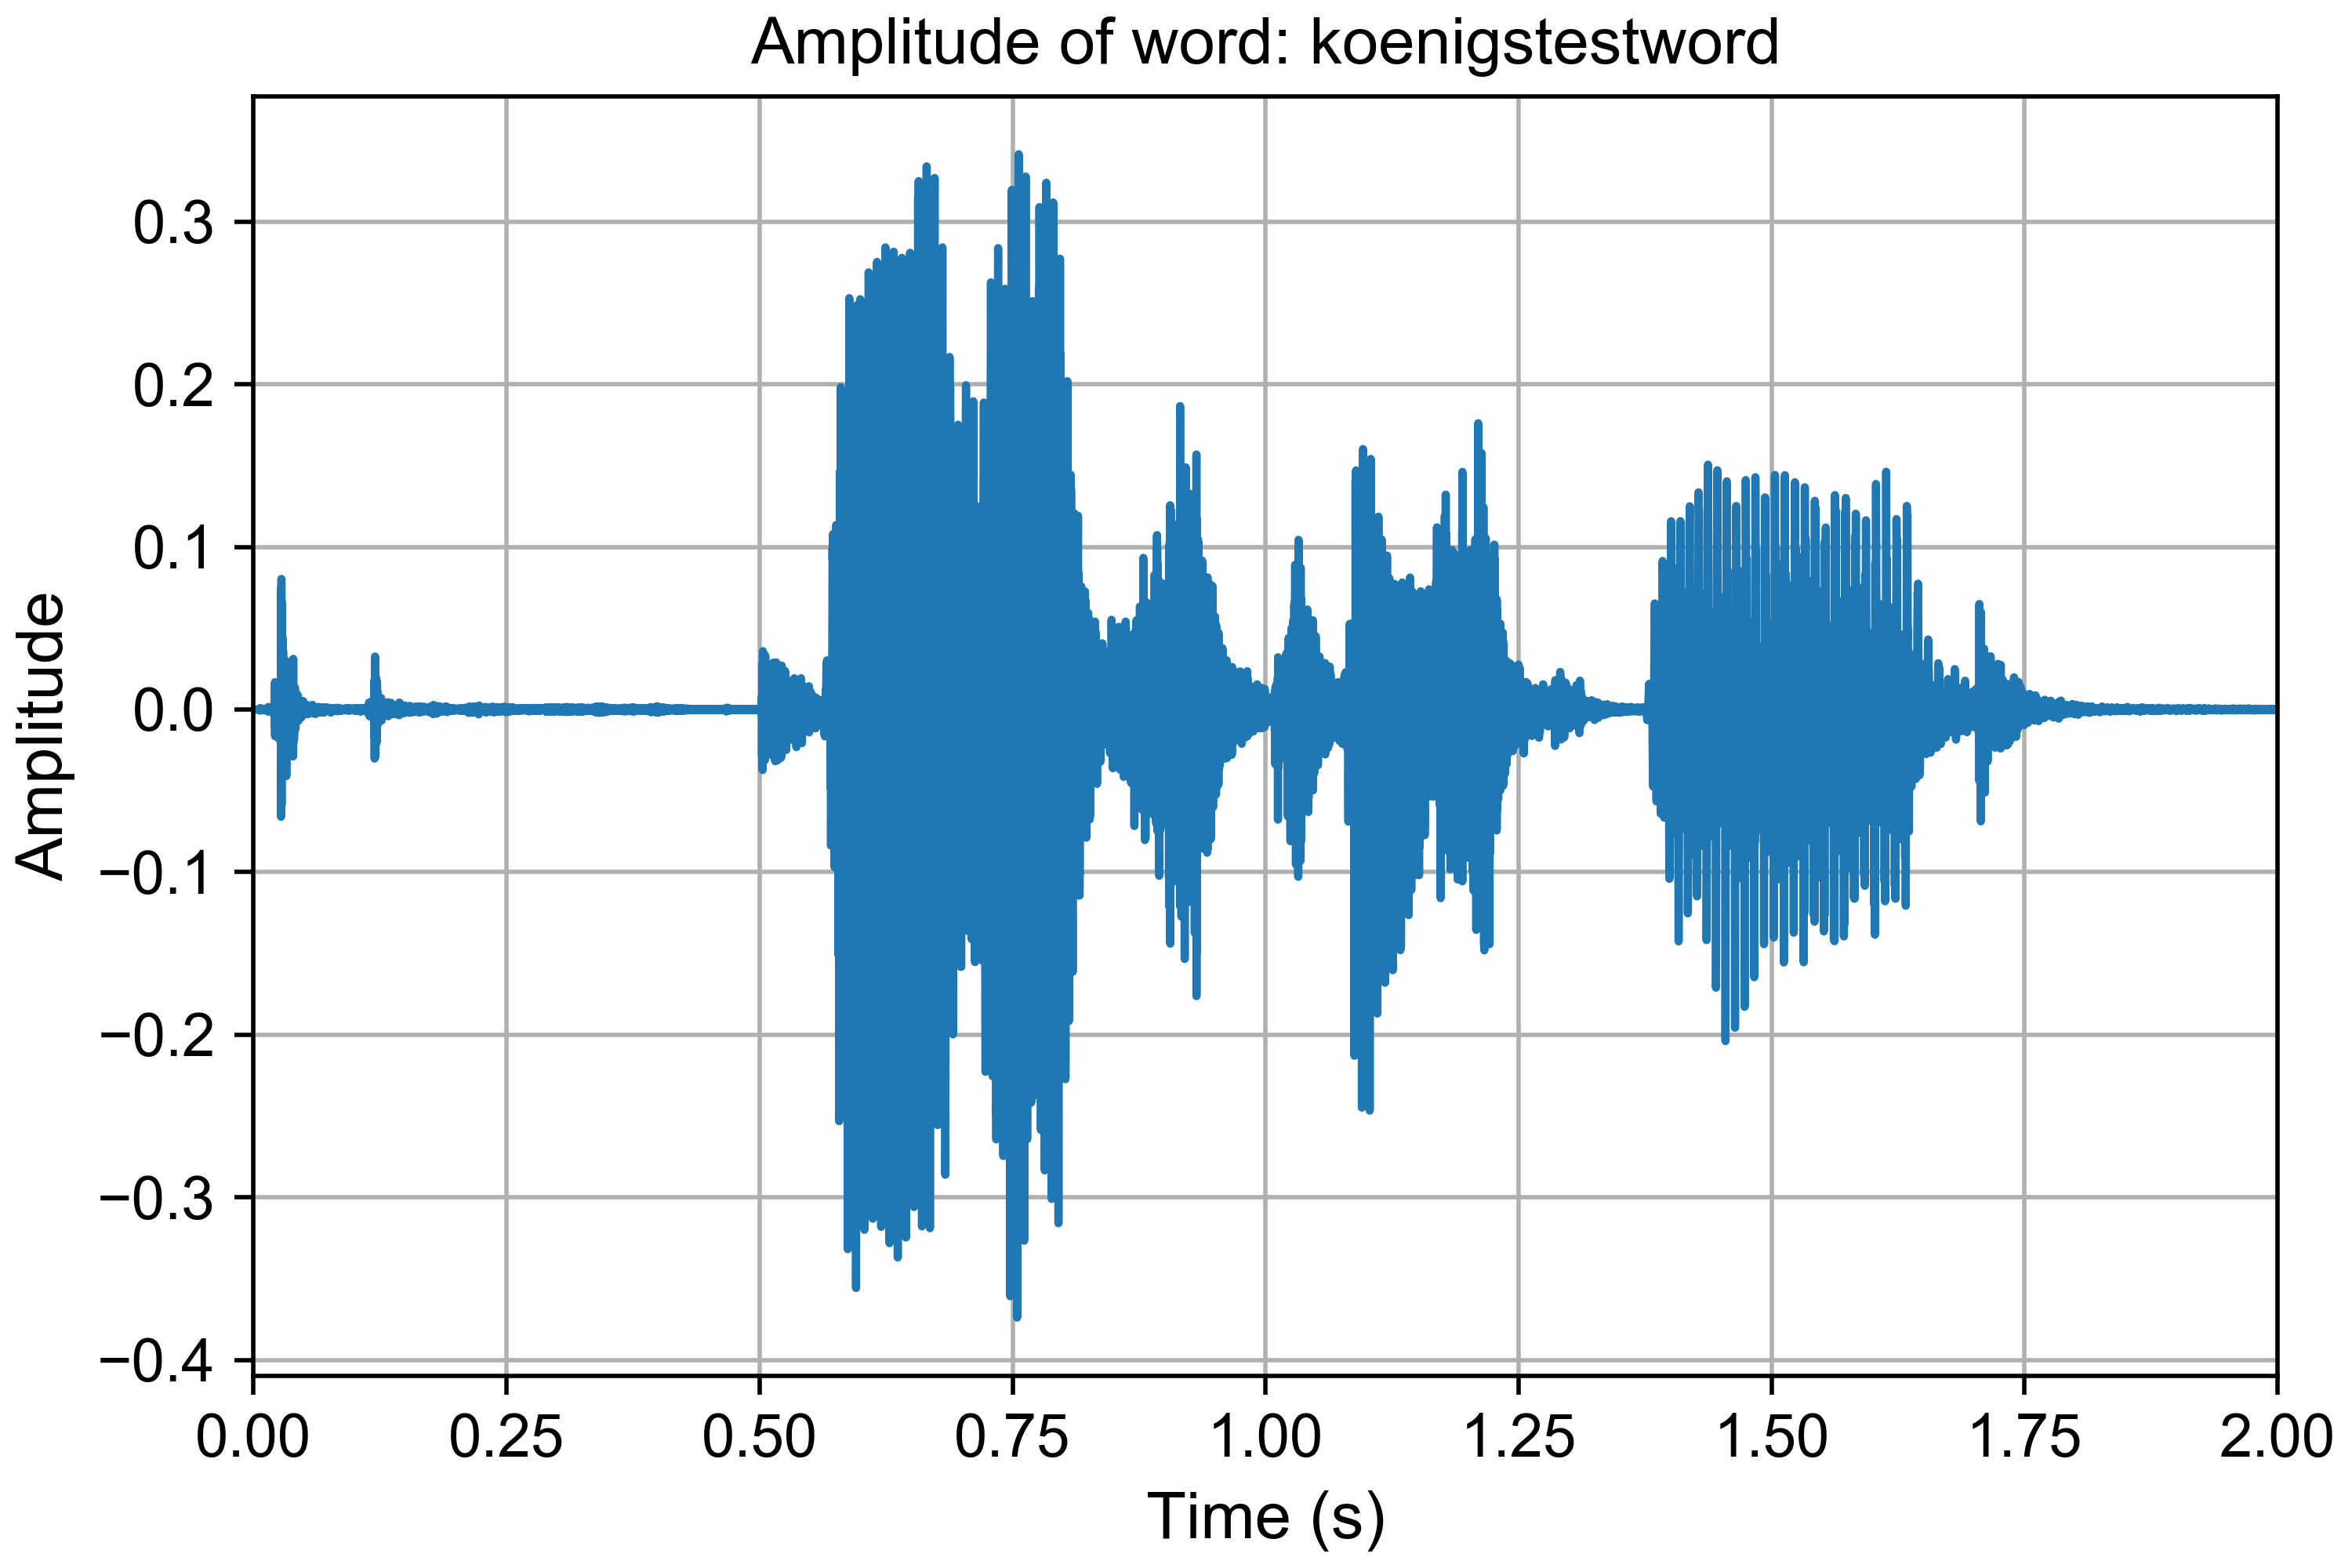
\includegraphics[width=0.8\textwidth]{figures/amplitude_koenigstestword}
	\caption{Amplitude of original signal}
	\label{fig:amplitude_koenigstestword}
\end{figure}
\begin{figure}[h]
	\centering
	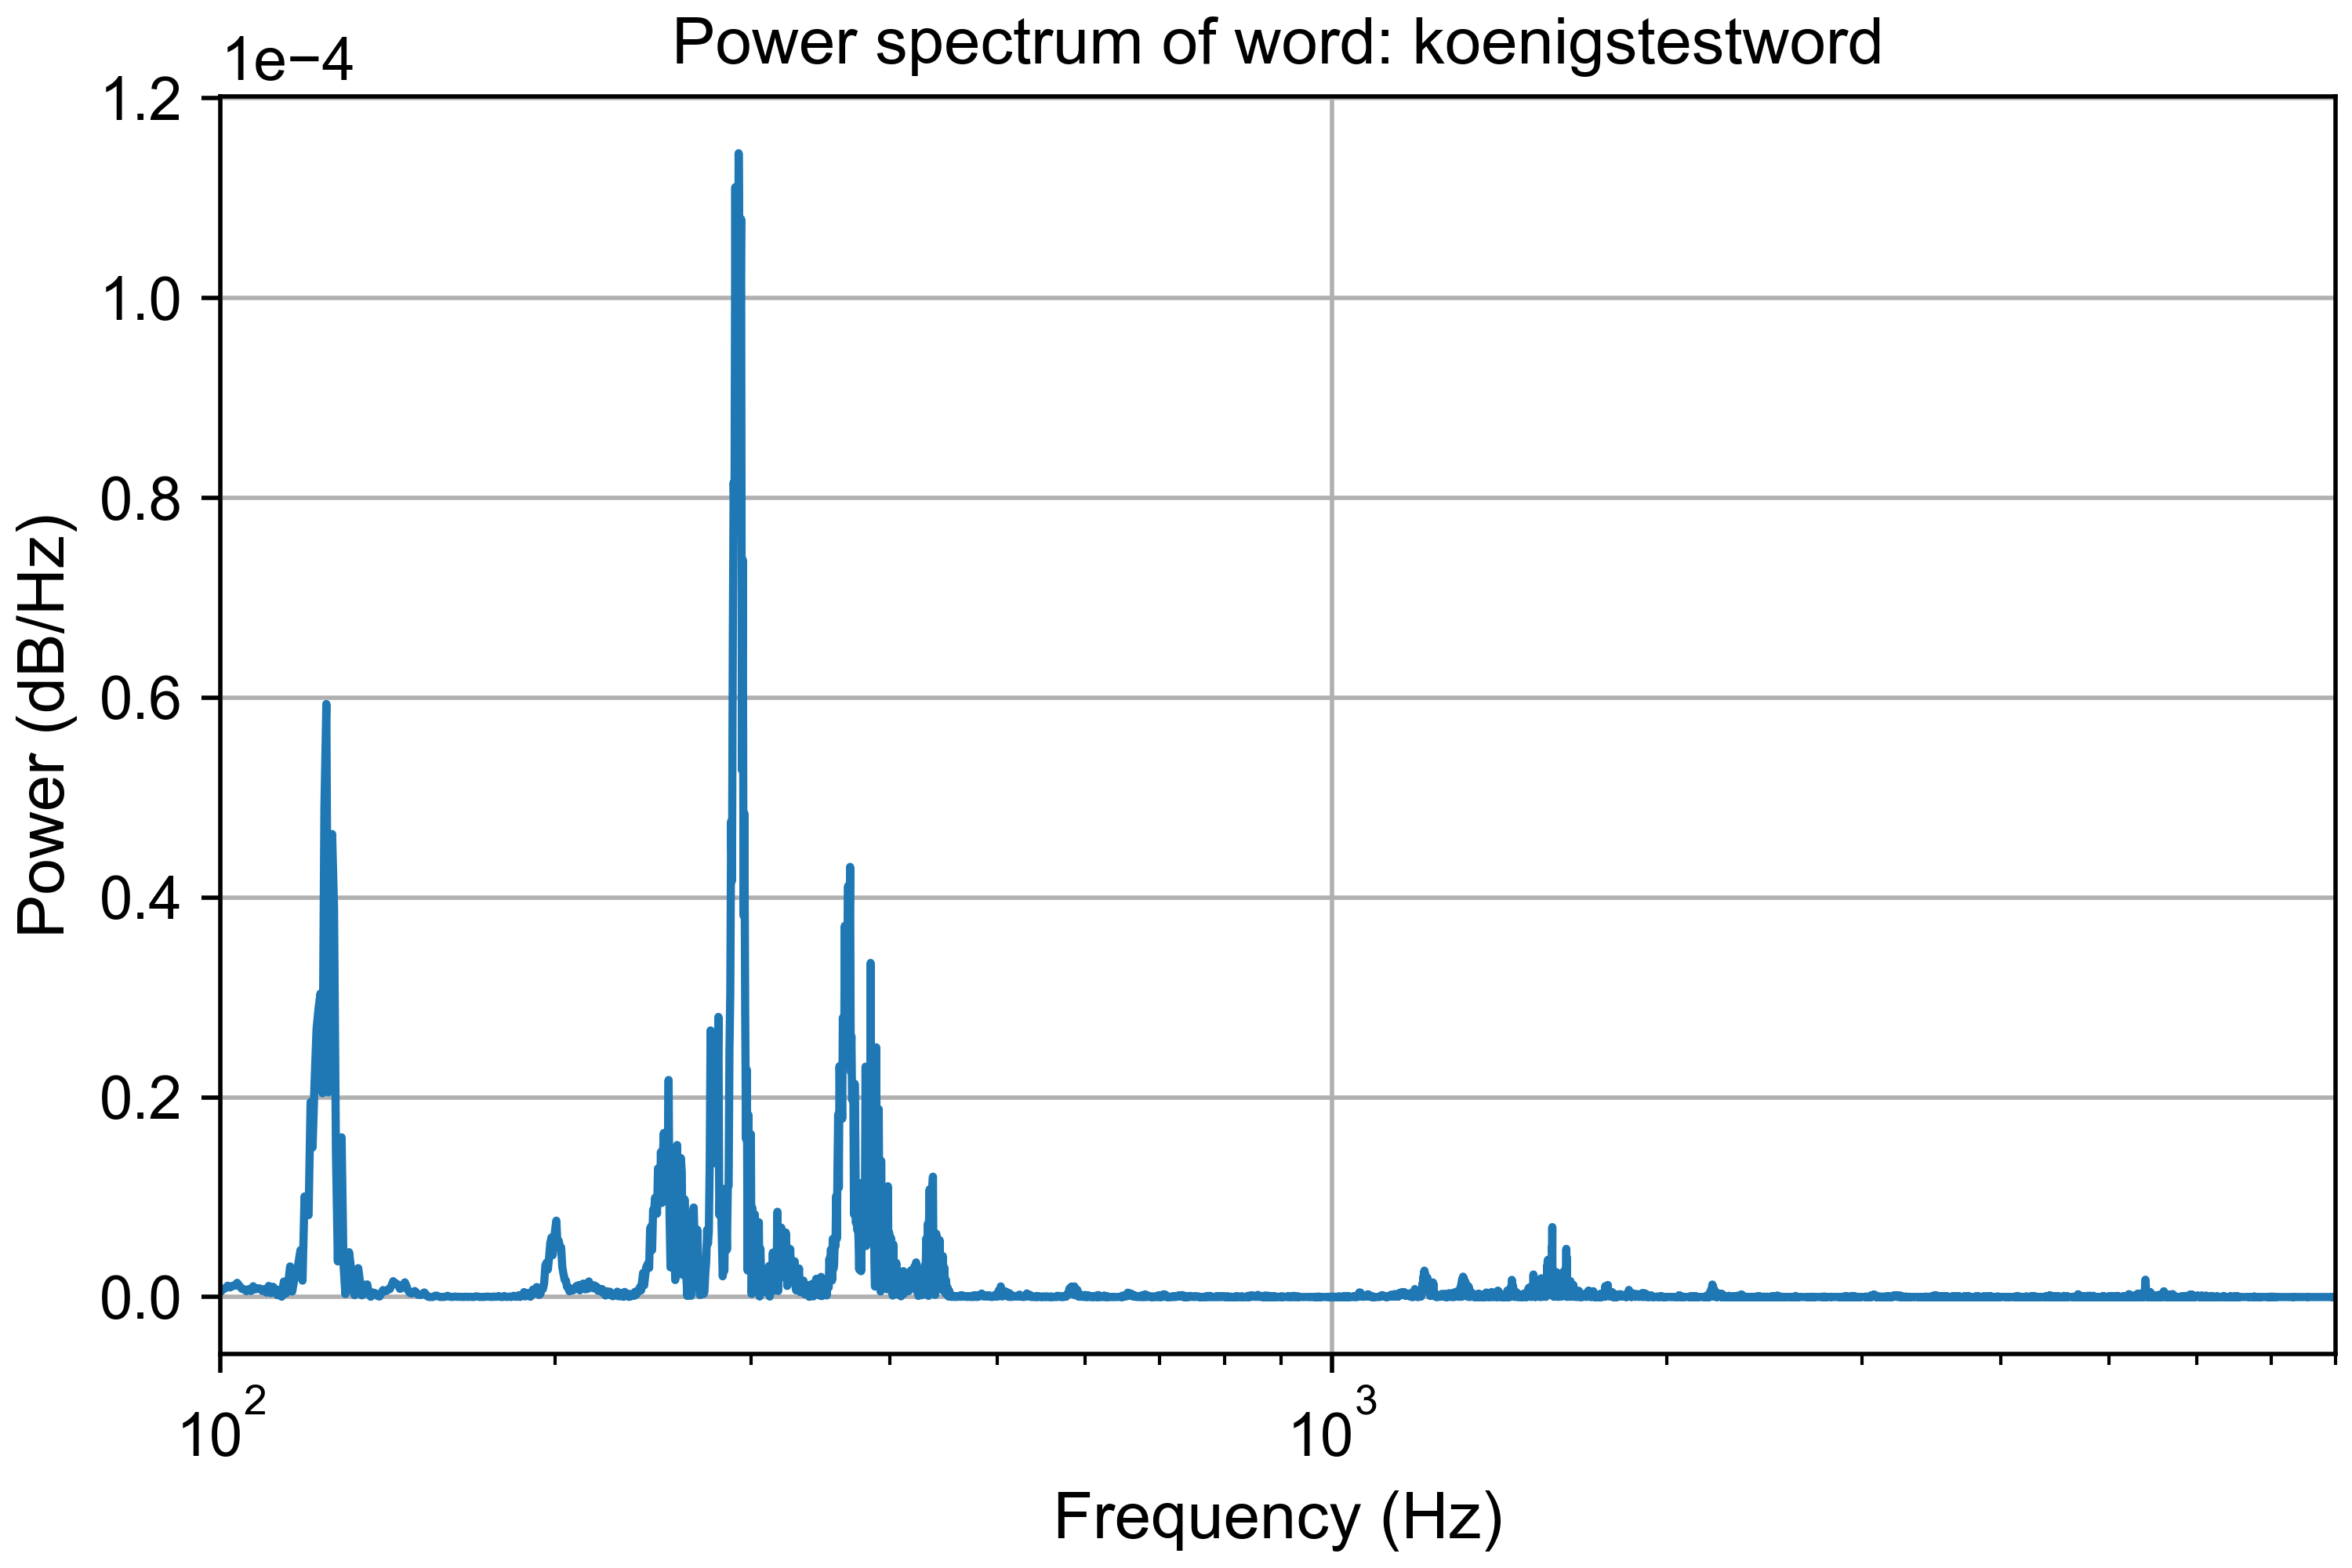
\includegraphics[width=0.8\textwidth]{figures/spectrum_koenigstestword}
	\caption{Power spectrum of original signal}
	\label{fig:spectrum_koenigstestword}
\end{figure}
\begin{figure}[h]
	\centering
	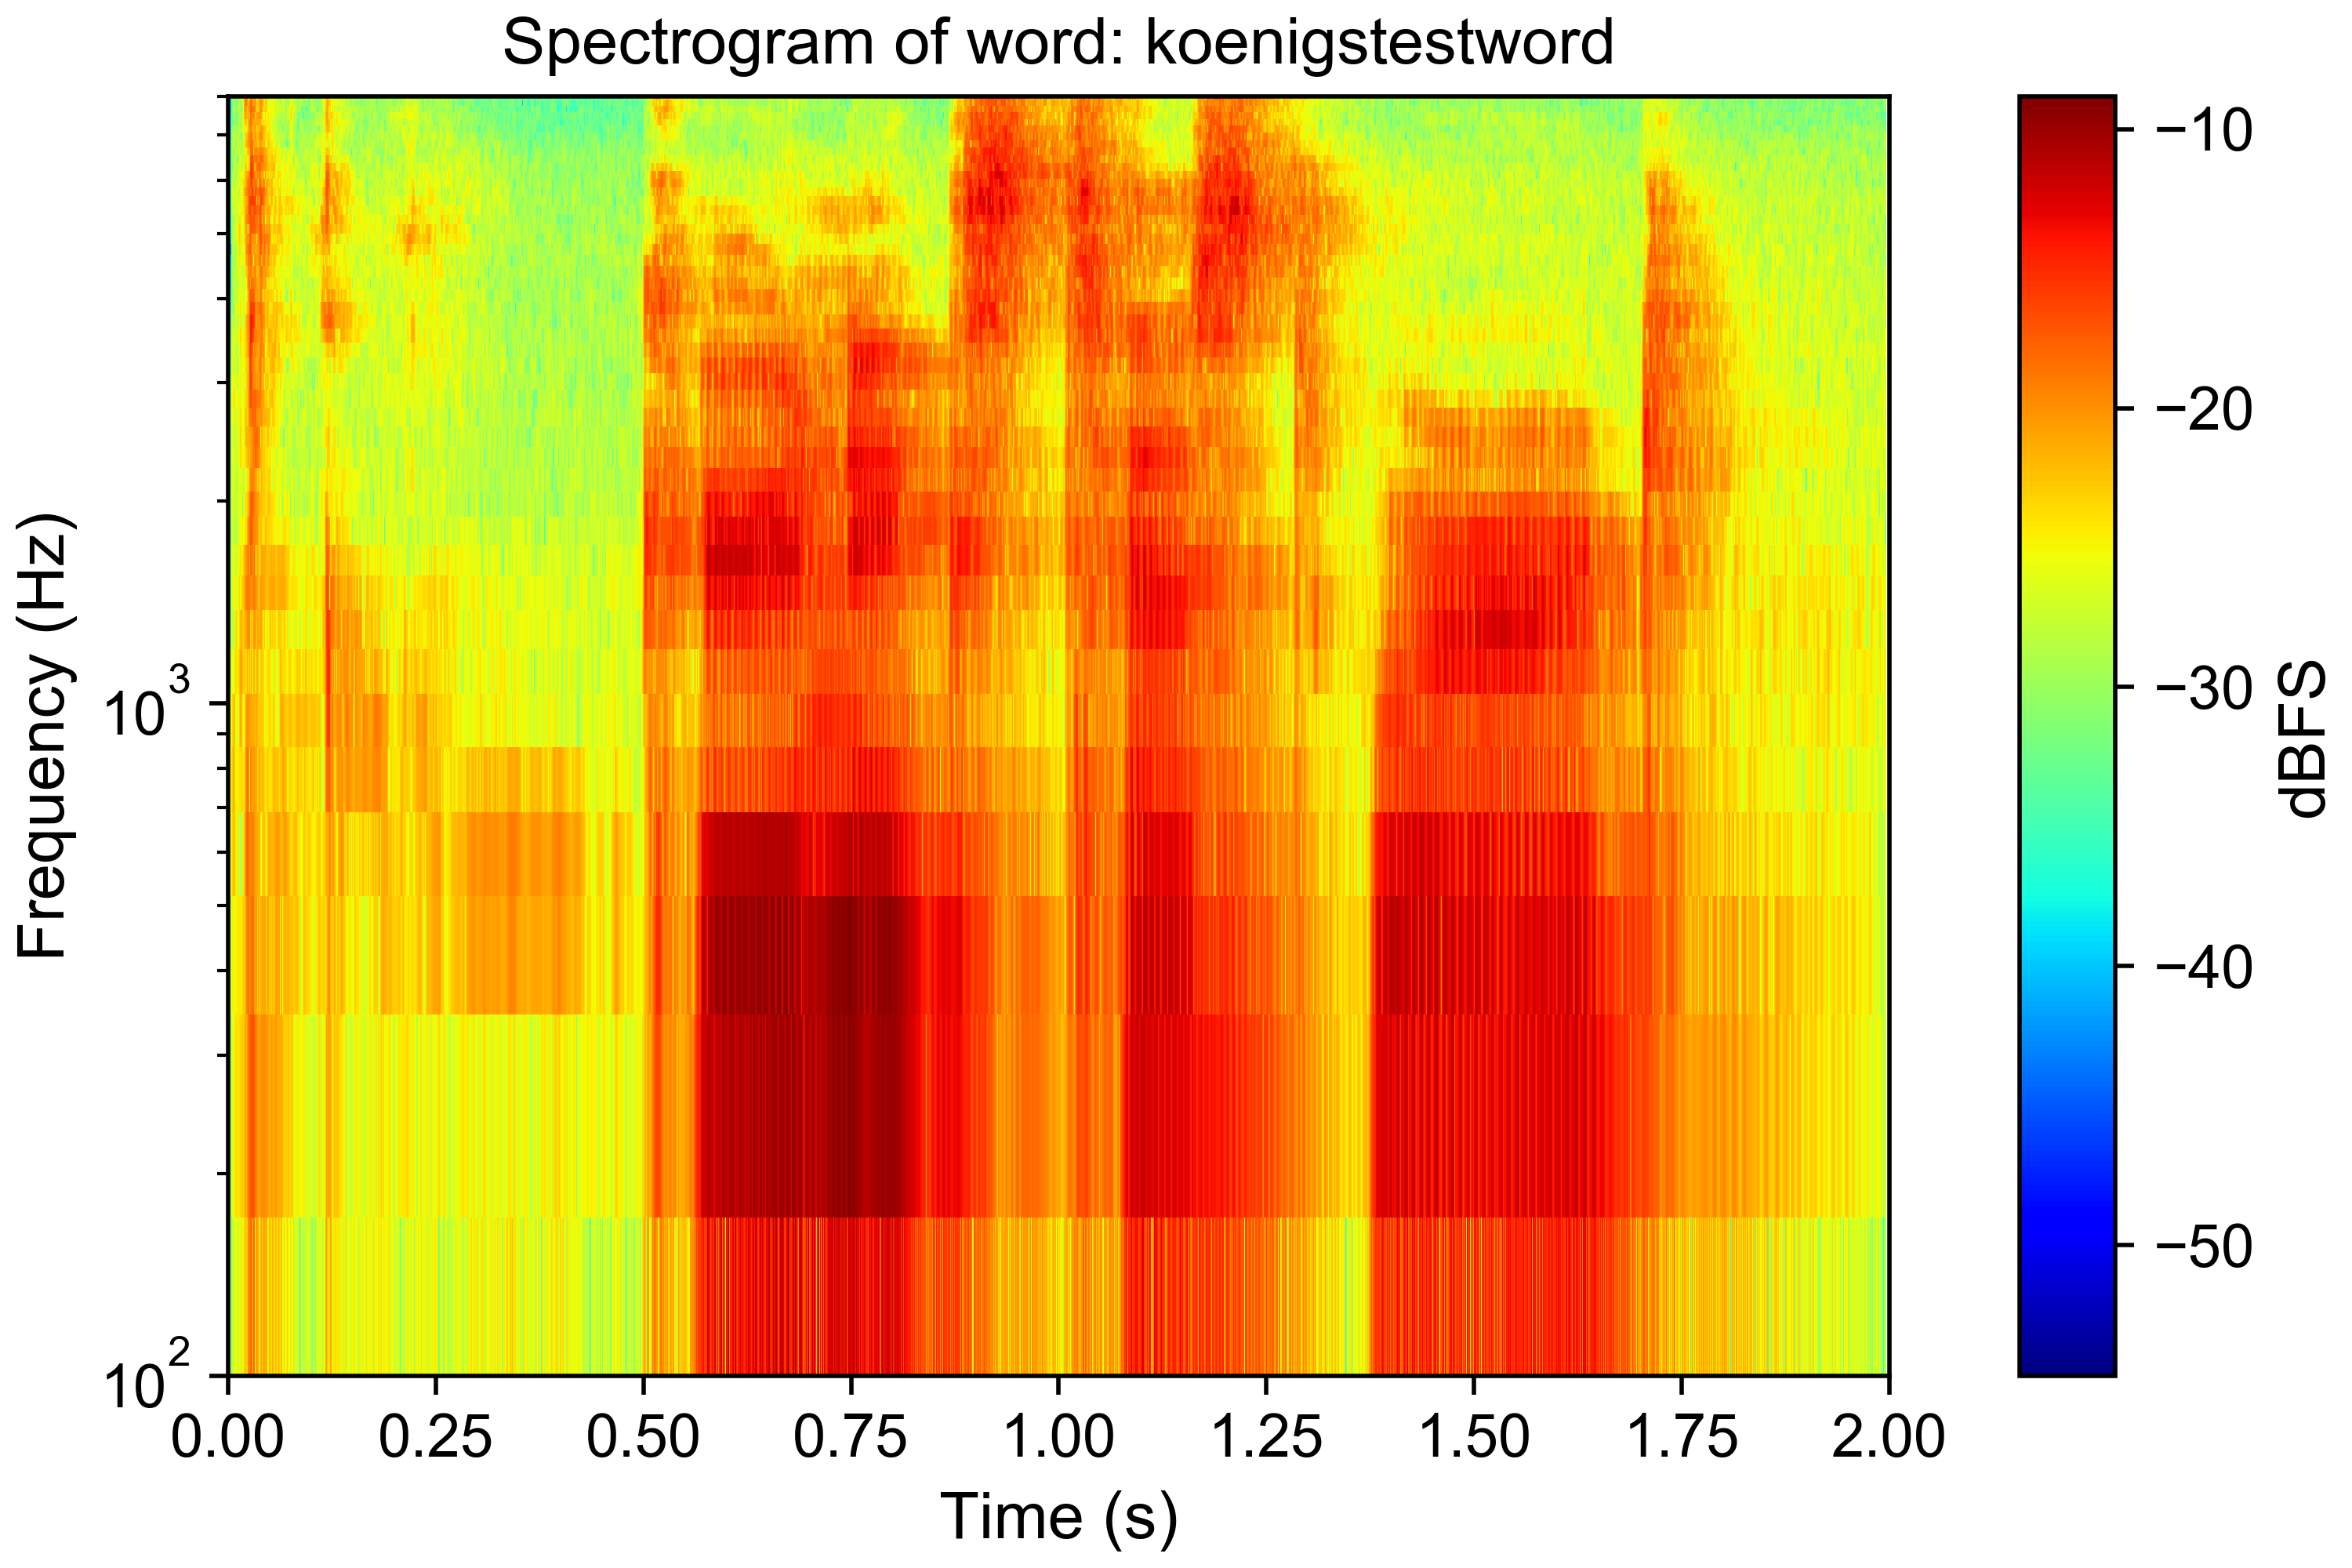
\includegraphics[width=0.8\textwidth]{figures/spectrogram_koenigstestword}
	\caption{Spectrogram of original signal}
	\label{fig:spectrogram_koenigstestword}
\end{figure}


\begin{figure}[p]
	\centering
	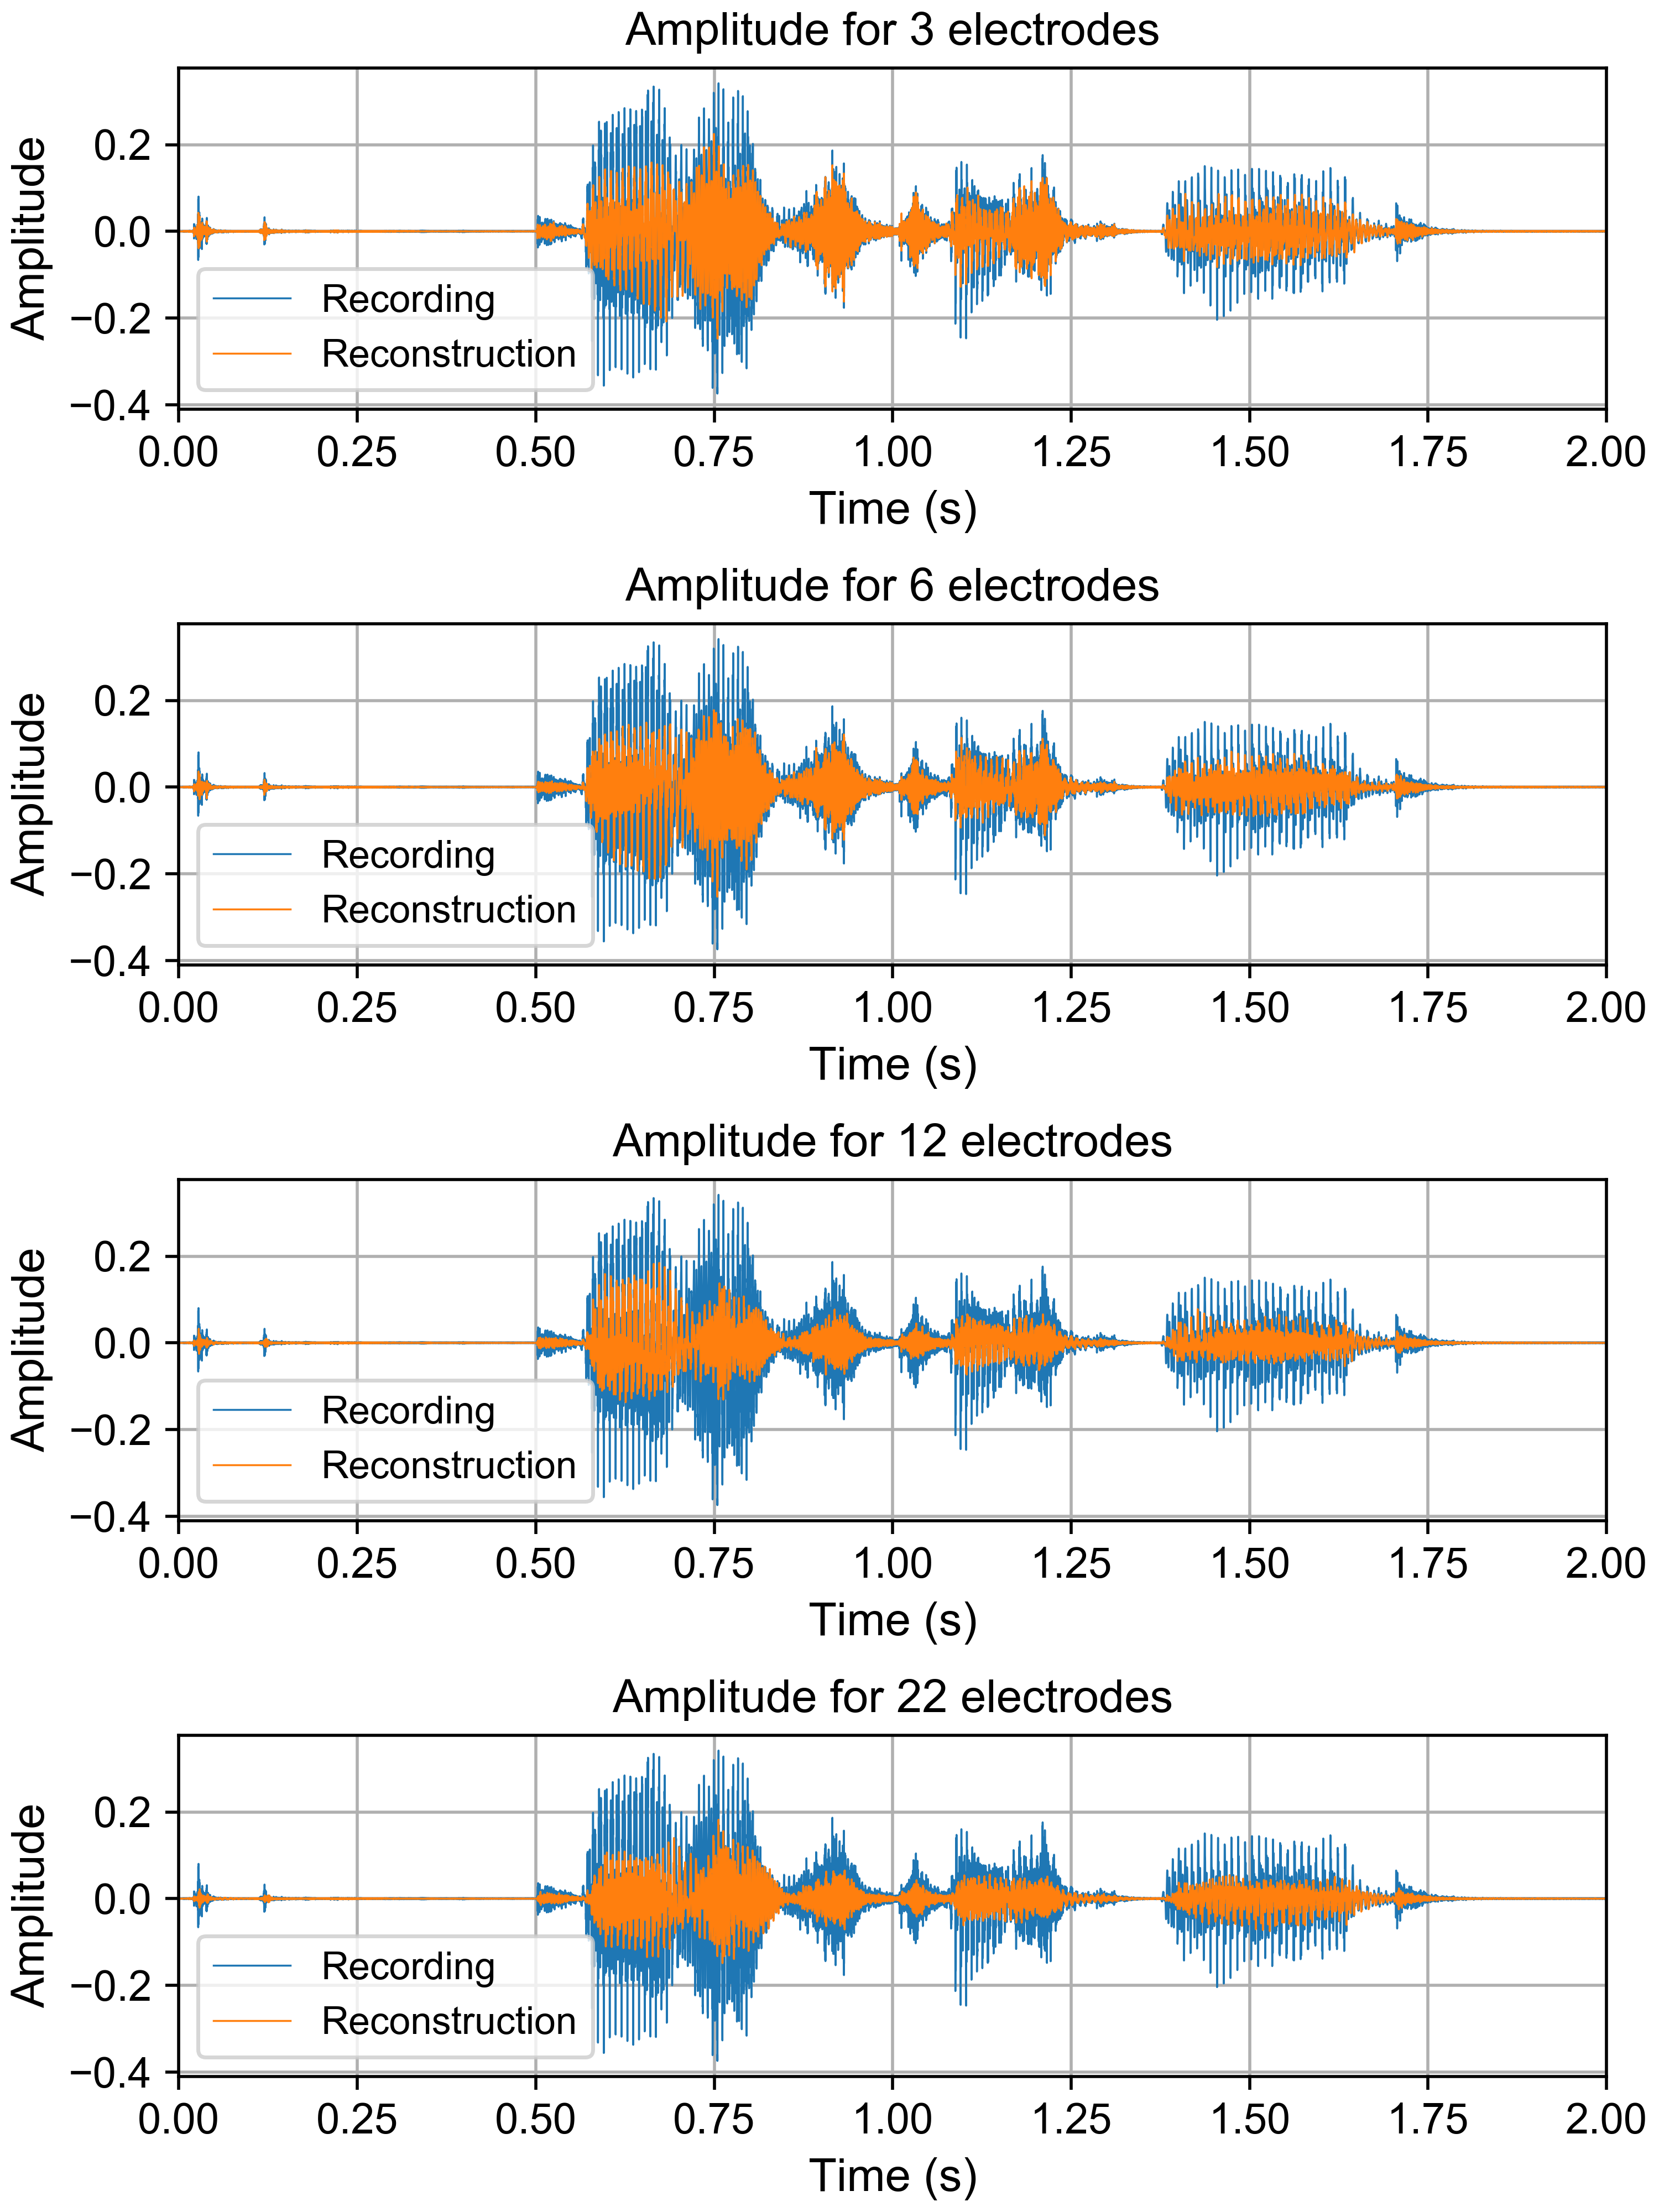
\includegraphics[width=0.8\textwidth]{figures/amplitude_sum}
	\caption{Amplitude of the summed signals for each CI}
	\label{fig:amplitude_sum}
\end{figure}
\begin{figure}[p]
	\centering
	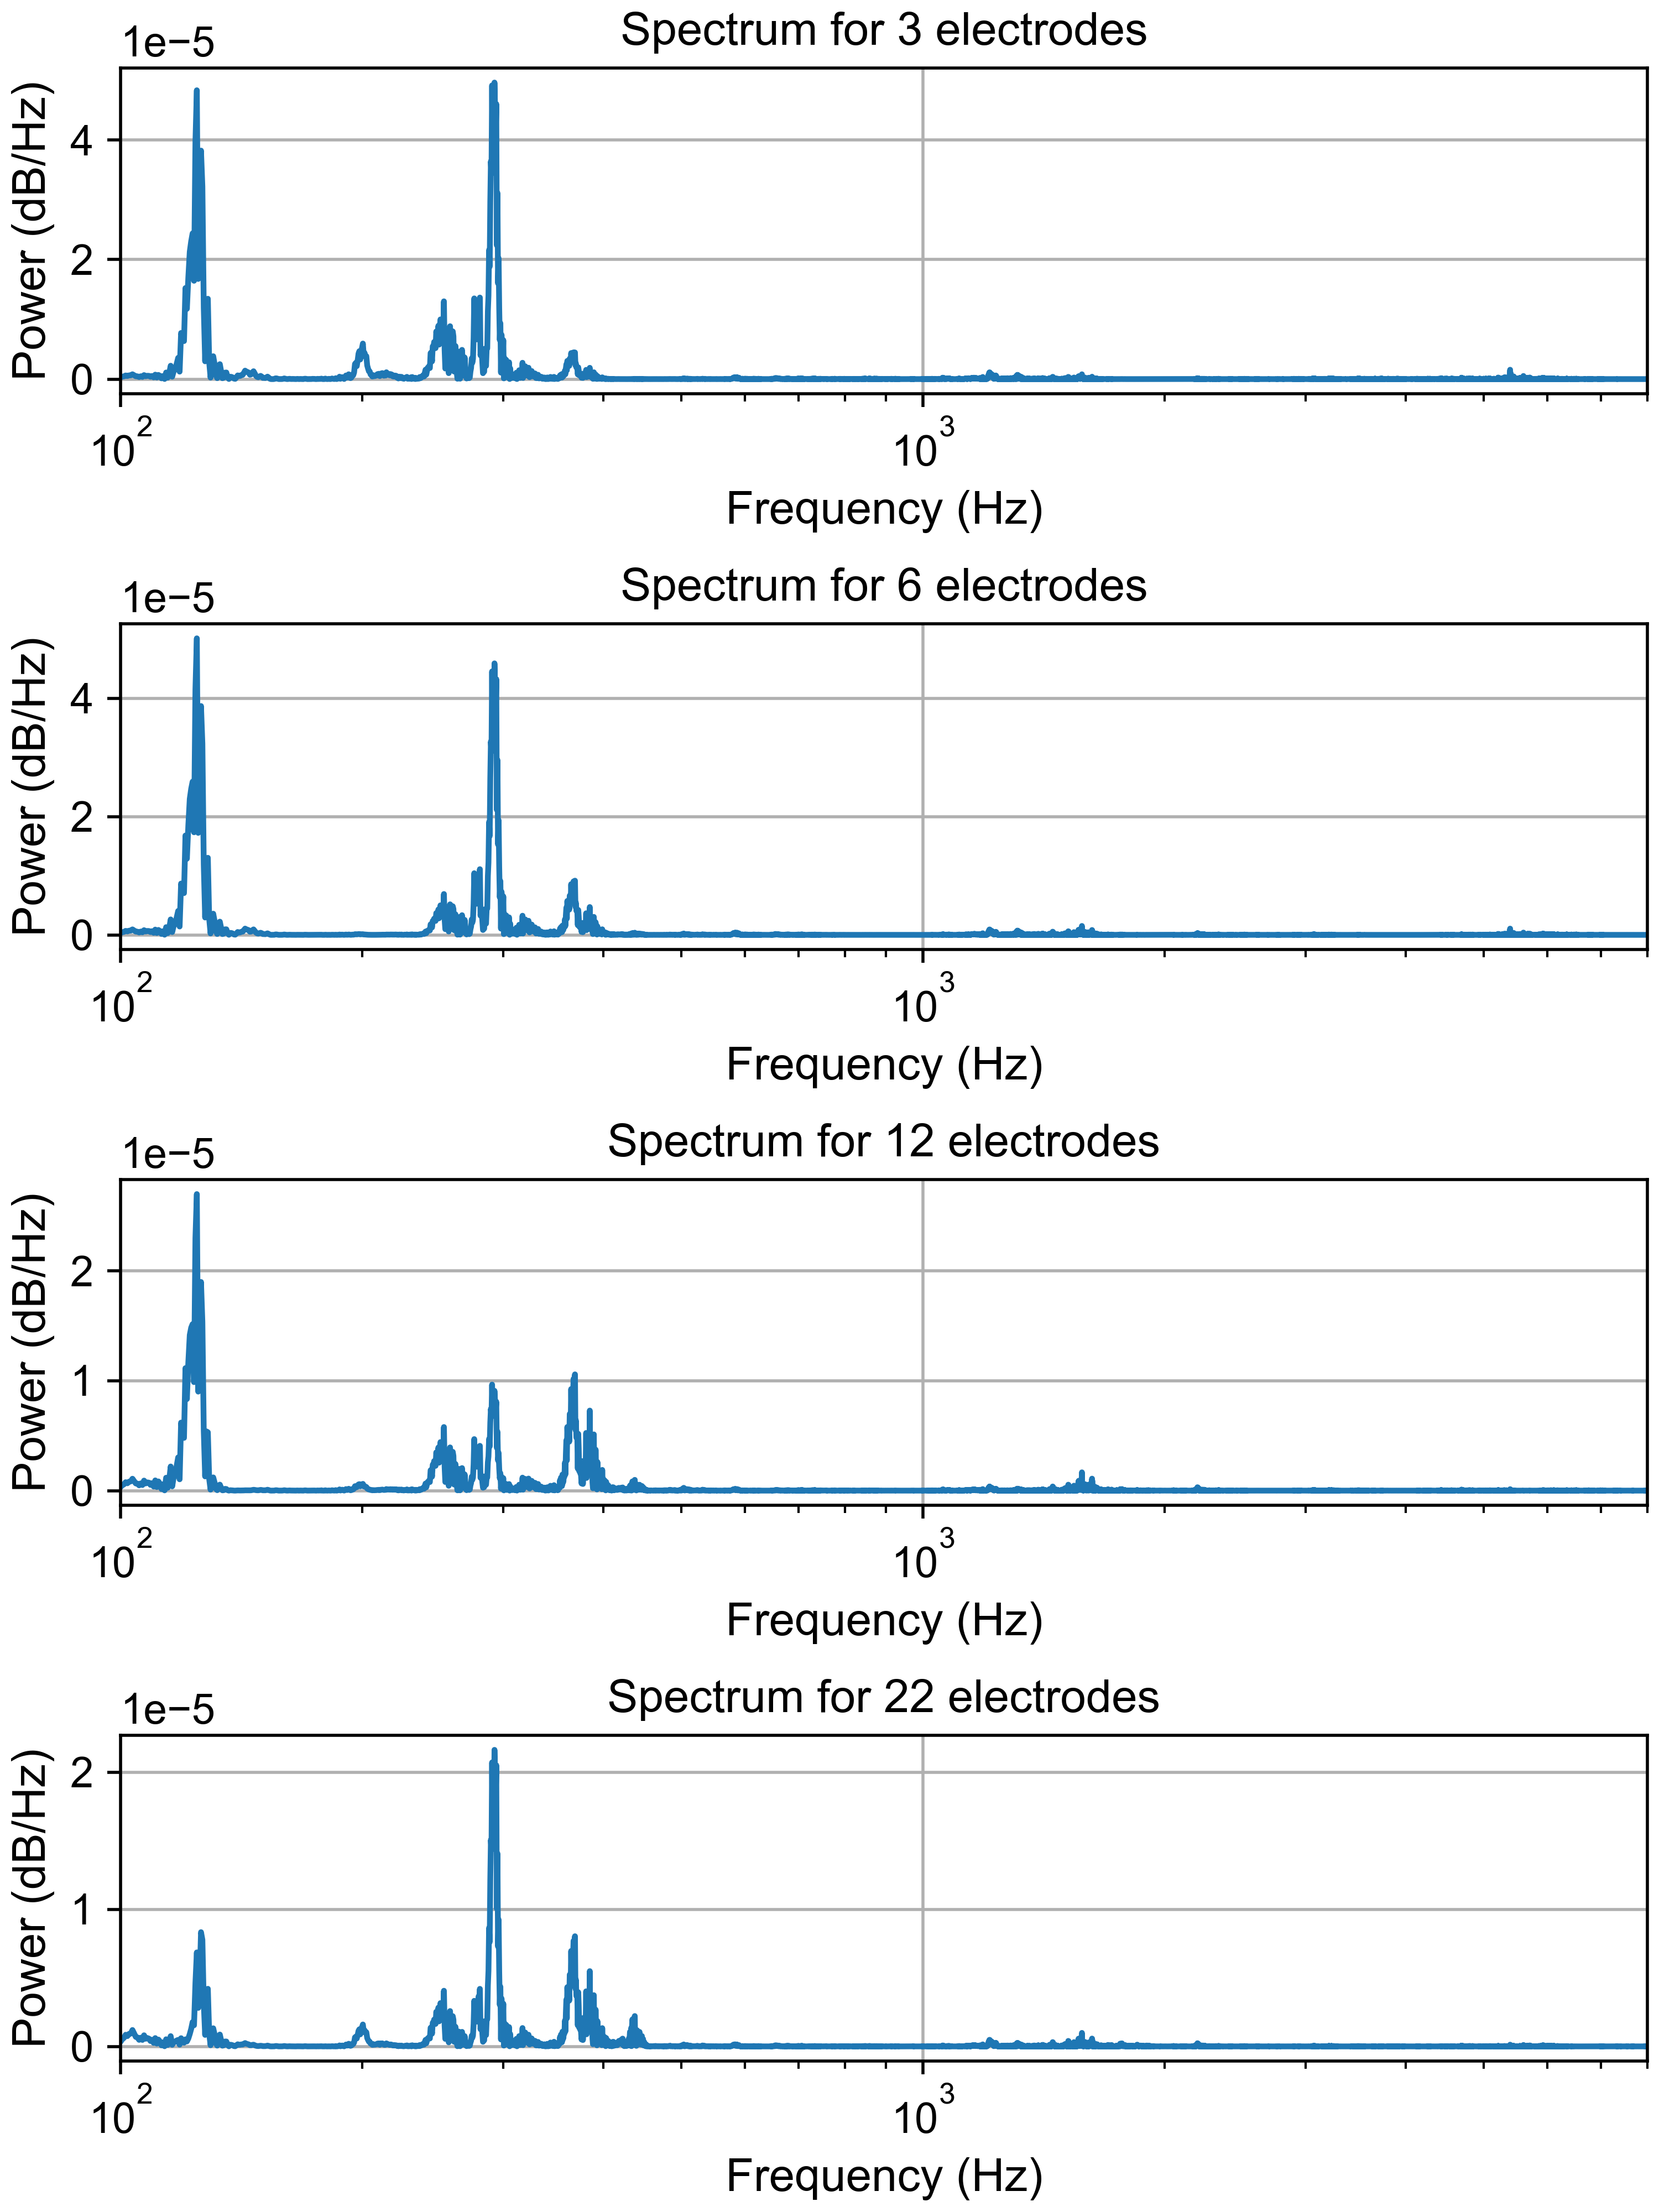
\includegraphics[width=0.8\textwidth]{figures/spectra}
	\caption{Power spectra of the summed signals for each CI}
	\label{fig:spectra}
\end{figure}
\begin{figure}[p]
	\centering
	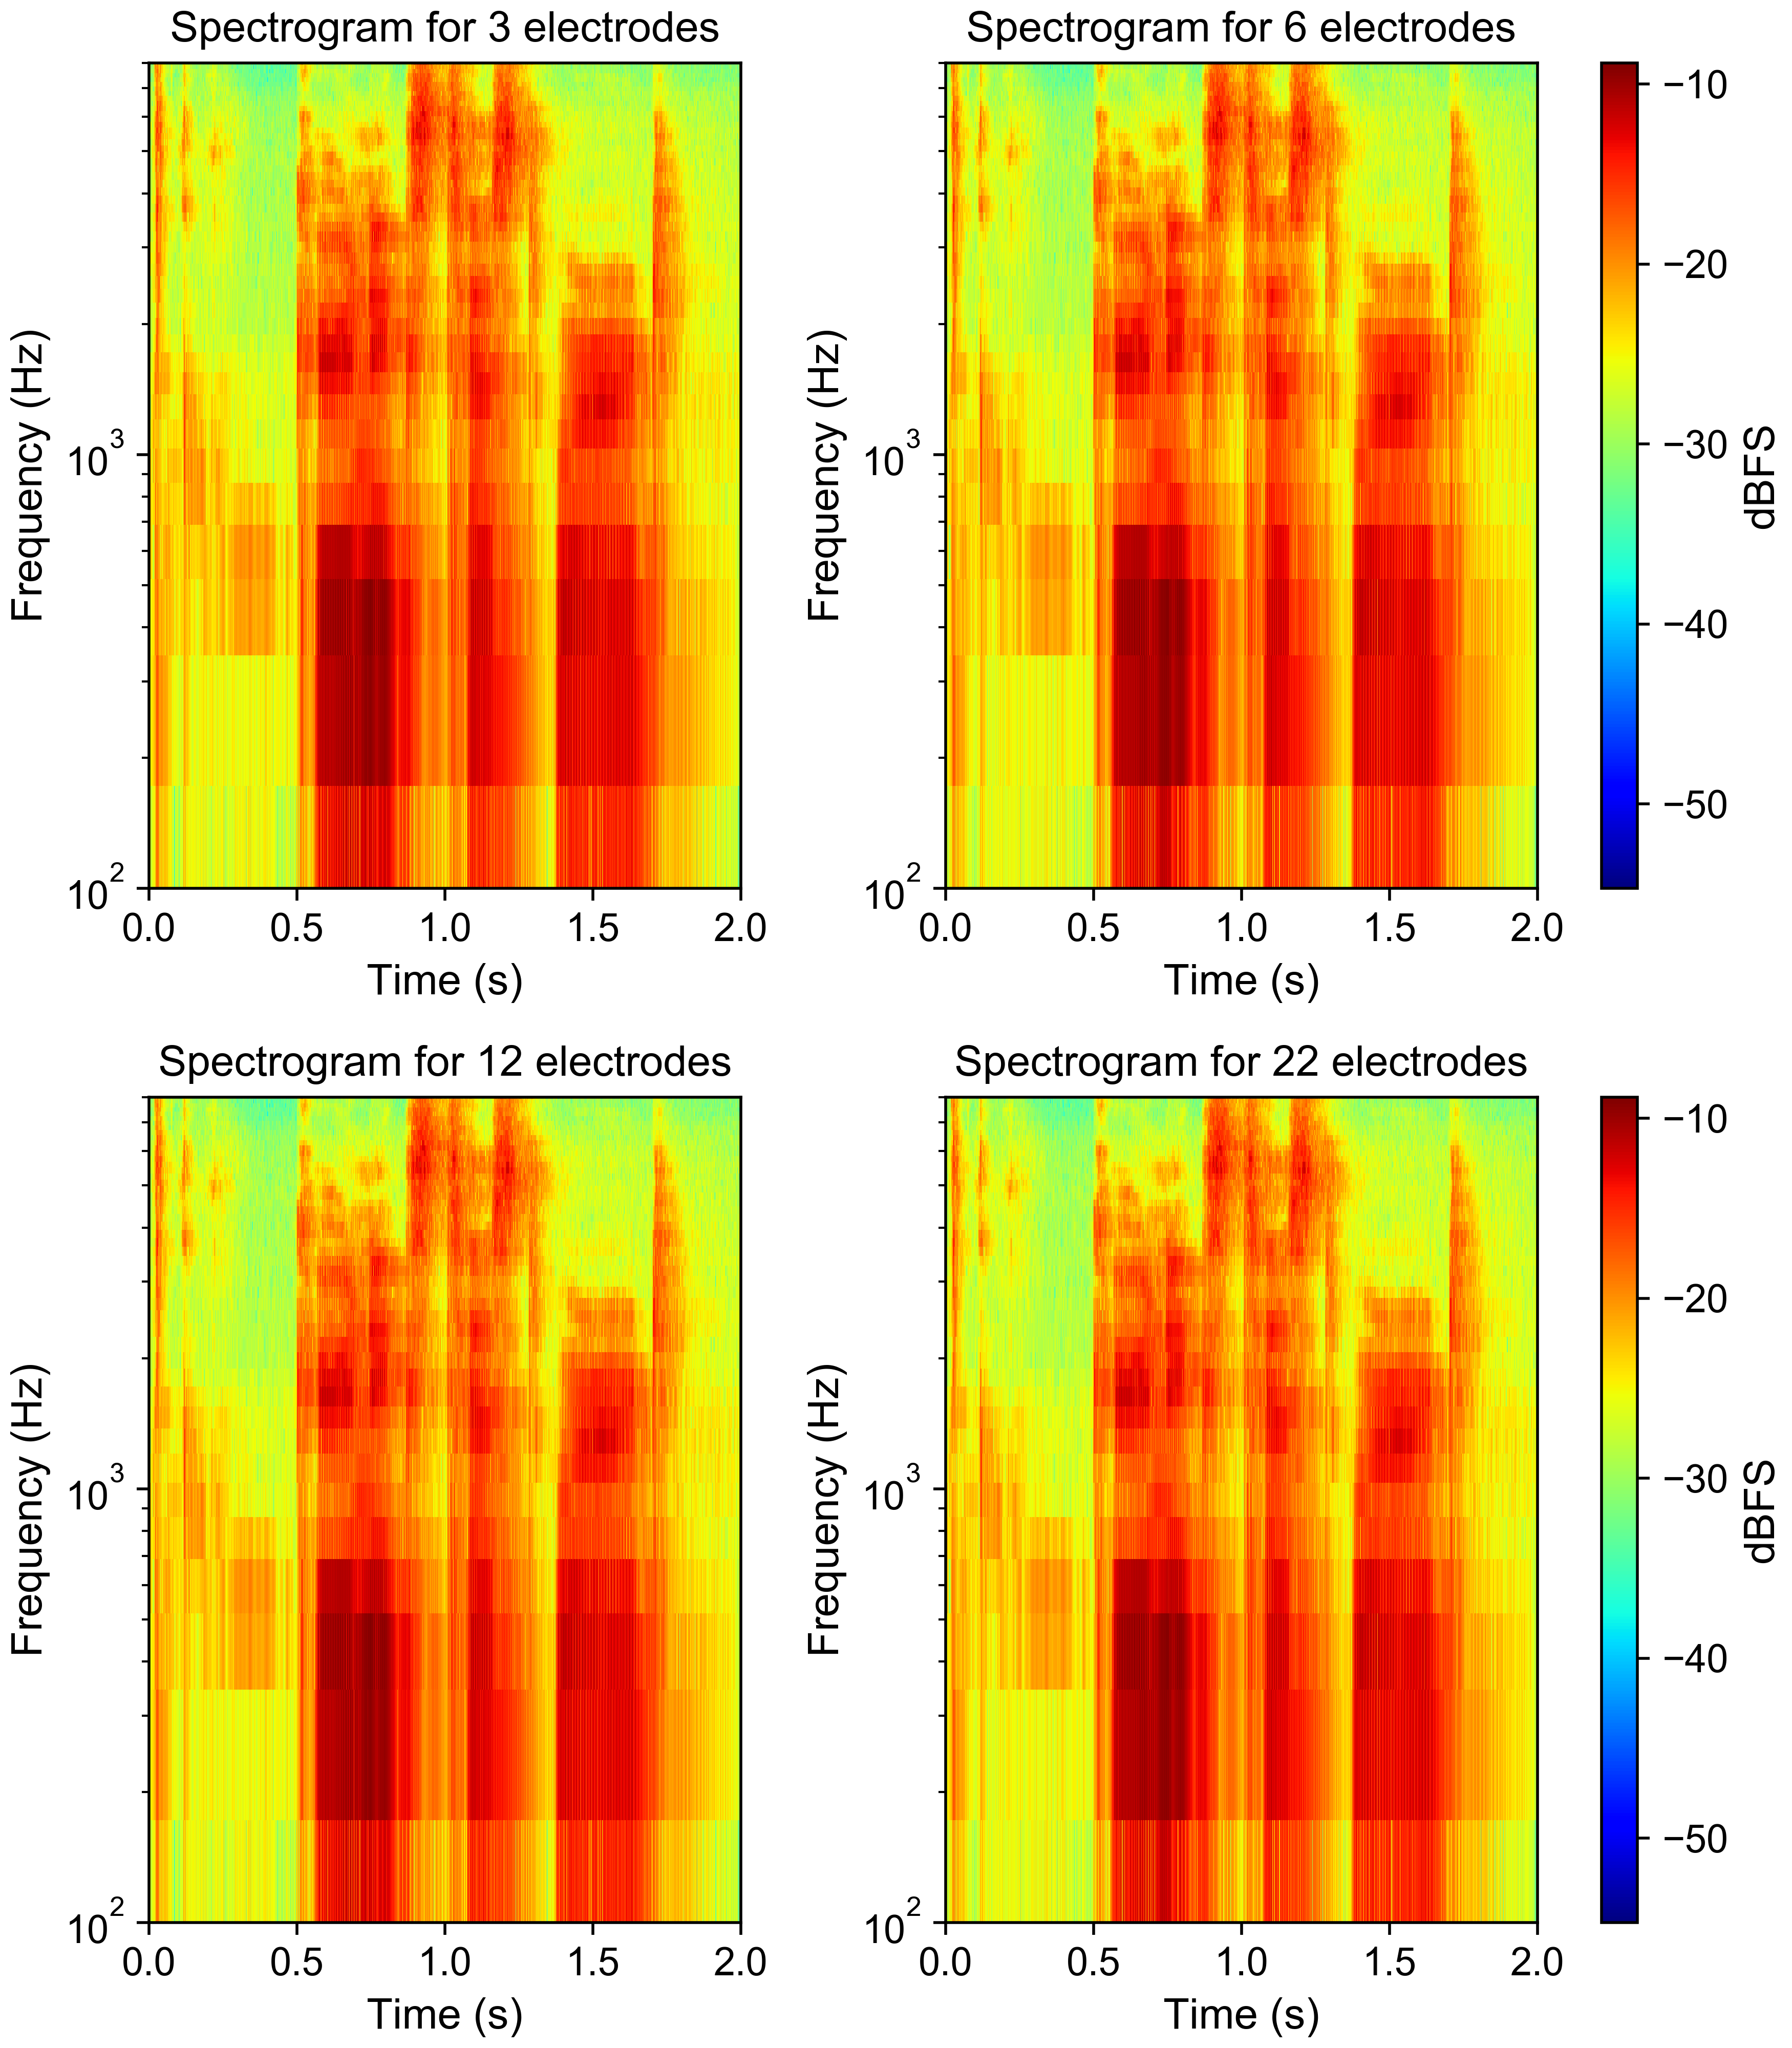
\includegraphics[width=0.8\textwidth]{figures/spectrograms}
	\caption{Spectrograms of the summed signals for each CI}
	\label{fig:spectrograms}
\end{figure}


\end{document}